\documentclass[a4paper,dutch,11pt,]{scrartcl}
\usepackage{mystyle}

\title{Simulated Annealing voor TTP (TTSA)}
\subtitle{Capita selecta computerwetenschappen: Artificiële intelligentie (|H05N0a|)}
\author{Philippe Tanghe \and Li Quan}
%\subject{Verslag}
\date{16 maart 2011}
\bibliographystyle{abbrv}


\begin{document}
\maketitle

%\begin{abstract}

%\end{abstract}

\tableofcontents

\section{Inleiding}
Dit verslag behandelt het traveling tournament problem (TTP). Hierbij worden optimale sport schedules gezocht die voldoen aan bepaalde constraints~\cite{ttp}.
De gekozen paper is van Anagnostopoulos, Van Hentenryck, Michel en Vergados~\cite{paper}: hun aanpak is gebaseerd op simulated annealing (SA) zoals oorspronkelijk beschreven in~\cite{simulatedannealing}, met enkele uitbreidingen zoals reheating en strategic oscillation. Additioneel is er ook de paper van Van Hentenryck en Vergados die de bovenstaande paper evalueert en uitbreidt naar niet NL-instanties~\cite{paper2}.

De reden voor de keuze van de paper is drievoudig:
\begin{enumerate}
 \item Uit de literatuur blijkt dat SA een van de betere metaheuristieken is voor het TTP~\cite{heuristicApproach}. De meerdere resultaten van de auteurs op de website~\cite{website} tonen dit ook aan.
 \item De gekozen paper beschrijft de gebruikte werkwijze duidelijk en concreet.
 \item Een van de personen die meegewerkt hebben aan de paper, namelijk Pascal Van Hentenryck, is een Belg.
\end{enumerate}

In dit verslag bespreken we eerst kort het probleem, de methode en de verschillende parameters, onze eigen implementatie en de moeilijkheden hierbij. We vergelijken onze resultaten met die in de paper en de website~\cite{website}. Ten slotte geven we mogelijke verbeteringen die onderzocht kunnen worden.

\section{Probleembeschrijving}
Voor een meer gedetailleerde beschrijving van het TTP wordt verwezen naar \cite{paper,ttp}.

\begin{description}
 \item[Input] $n$ teams ($n$ even) en een $n\times{}n$ symmetrische afstandsmatrix $D$, waarbij het element $d_{ij}$ de afstand tussen team $T_i$ en $T_j$ is.
 \item[Output] Een double round-robin tournament schema (= schedule).
\end{description}

Een double-round robin tournament is een toernooi waarbij elk team exact tweemaal kampt tegen elk ander team, namelijk eenmaal thuis en eenmaal uit.
De kost van een team is de totale afstand die het team moet afleggen.
De totale kost is dan de som van de kost van alle teams (waarbij elk team thuis start en eindigt). 

Er wordt dus gezocht naar een schedule met minimale afstandskost en die voldoet aan de atmost en norepeat constraints.
De atmost constraints houden in dat elk team maximaal drie keer opeenvolgend thuis of uit mag spelen; de norepeat constraints dat een wedstrijd $T_i$ uit bij $T_j$ niet onmiddellijk mag gevolgd worden door de wedstrijd $T_i$ thuis versus $T_j$.

Een schedule wordt voorgesteld door een tabel die de tegenstander van elk team weergeeft. De rijen stellen hierbij de teams voor; de kolommen de ronden.
De tegenstander van team $T_i$ in ronde $r_k$ wordt gegeven door de absolute waarde van het element $(i,k)$. Indien $(i,k)$ positief is, speelt $T_i$ thuis; anders op verplaatsing.

% Neem als voorbeeld volgend schedule $S$ voor 6 teams.
% \begin{center}
% \begin{tabular}{c | *{10}{r} }
%  \textbf{T\textbackslash{}R} & 1 & 2 &3 & 4 & 5 & 6 & 7 & 8 & 9 & 10 \\ \hline
% 1 &     6&-2&4&3&-5&-4&-3&5&2&-6 \\
% 2 &    5&1&-3&-6&4&3&6&-4&-1&-5\\
% 3 &    -4&5&2&-1&6&-2&1&-6&-5&4\\
% 4 &    3&6&-1&-5&-2&1&5&2&-6&-3\\
% 5&    -2&-3&6&4&1&-6&-4&-1&3&2\\
% 6 &  -1&-4&-5&2&-3&5&-2&3&4&1 \\
% \end{tabular}
% \end{center}



%Om een uitwedstrijd voor te stellen wordt een minteken geplaatst voor het team waartegen gespeeld wordt.
%Het schedule wordt voorgesteld door een matrix, waarin de rijen de teams voorstellen waartegen het team, overeenkomstig met die rij, moet spelen. De kolommen stellen de opeenvolgende ronden voor.
%
\section{Simulated annealing}
Het oorspronkelijke algemene simulated annealing~\cite{metaheuristics,simulatedannealing} wordt hier niet verder besproken. 
Het voorgestelde simulated annealing algoritme voor het TTP (TTSA) heeft volgende belangrijke karakteristieken~\cite{paper}:

\begin{enumerate}
\item TTSA deelt de constraints op in hard (geldig double round-robin tournament) en soft constraints (atmost en de norepeat constraints).
\item TTSA heeft een nabuurschap (neighborhood) van grootte $\mathcal{O}(n^3)$.
\item TTSA bevat een strategic oscillation strategie om de tijd die doorgebracht wordt in de feasible en infeasible oplossingen te balanceren.
\item TTSA gebruikt het concept van `reheats' om uit locale minima te geraken bij lage temperaturen.
\end{enumerate}
%
% Naast de reeds vermelde hard en soft constraints is het de bedoeling de oplossing te vinden die een minimale kost heeft. De kost wordt bepaald door de som van de afstanden die elk team moet afleggen doorheen het toernooi.

\subsection*{Initi\"ele oplossing}
TTSA begint vanuit een random gegenereerde schedule, die een double round-robin tournooi voorstelt. Deze wordt gevonden met een eenvoudige recursieve backtrack search.

\subsection*{Local search}
De basisstap is dat van een huidig schedule $S$ een schedule $S'$ gekozen wordt in de neighborhood. 
Indien het verschil tussen de nieuwe kost en de oude kost, $\Delta$, kleiner is dan 0, wordt $S'$ geaccepteerd; anders slechts met kans $\exp({-\Delta{}/T})$ (waarbij de temperatuur $T$ een controleparameter is).  Na een bepaald aantal iteraties wordt afgekoeld ($T\leftarrow\ T\cdot\beta$) waardoor de kans om slechtere oplossingen te kiezen, gradueel kleiner wordt.

\subsection*{Neighborhood}
Er zijn vijf mogelijke modificaties:
\begin{enumerate}
\item \emph{SwapHomes($S,T_i,T_j$)} wisselt in schedule $S$ de thuis- en uitrollen van teams $T_i$ en $T_j$.
\item \emph{SwapRounds($S,r_k,r_l$)} wisselt in schedule $S$ ronde $r_k$ met ronde $r_l$.
\item \emph{SwapTeams($S,T_i,T_j$)} wisselt in schedule $S$ het schema van team $T_i$ met dat van $T_j$ (behalve in de rondes waarin ze tegen elkaar spelen).
\item \emph{PartialSwapRounds($S,T_i,r_k,r_l$)} wisselt in schedule $S$ ronde $r_k$ met $r_l$ voor team $T_i$ en zorgt (op een deterministische wijze) dat het bekomen schema terug een double round-robin schema wordt.
\item \emph{PartialSwapTeams($S,T_i,T_j,r_k$)} wisselt in schedule $S$ de tegenstander van $T_i$ met die van $T_j$ in ronde $r_k$ en zorgt (op een determistische wijze) dat het bekomen schema terug een double round-robin schema wordt.

\end{enumerate}

\subsection*{Objectieffunctie}
De objectieffunctie $C$ van een schedule $S$ is als volgt gedefinieerd:
\begin{equation*}
  C(S)=%
  \begin{cases}
    cost(S) &\textrm{als $S$ feasible is,} \\
    \sqrt{cost(S)^2 + [w\cdot{}f(nbv(S))]^2} &\textrm{anders}.
  \end{cases}
\end{equation*} $cost(S)$ is de gewone afstandskost van een schedule, $nbv(S)$ duidt het aantal violations tegen de (soft) constraints van $S$ aan. $w$ is een gewichtsfactor en $f$ een sublineaire functie waarbij $f(1)=1$. Het doel van deze laatste functie is om de eerste violation kostelijker te maken dan de volgende. In de oorspronkelijke paper\footnote{In~\cite{paper2} wordt dit echter verfijnd naar $f(v)=1+(\sqrt{v}\ln{v})/\lambda$, met $\lambda=2$ voor kleine instanties en $\lambda=1$ voor grotere instanties. In onze experimenten werd steeds de oorspronkelijke versie gebruikt.} wordt gebruik gemaakt van $f(v)=1+(\sqrt{v}\ln{v})/2$.

\subsubsection*{Strategic Oscillation}
De gewichtsfactor $w$ wordt gebruikt om de zoektocht te leiden langs feasible dan wel infeasible schedules. Wanneer TTSA een nieuwe beste oplossing vindt, wordt $w$ vermenigvuldigd met $\delta$ als het een infeasible schedule is en indien feasible, gedeeld door $\theta$ (waarbij $\delta$ en $\theta$ $>1$). In de paper wordt $\delta{}=\theta{}=1.04$ gekozen.


\subsection*{Reheating}
TTSA kan moeilijk uit lokale minima ontsnappen op lage temperaturen. Daarom wordt een aantal keren de temperatuur opnieuw verhoogd.
We gebruiken een eenvoudig reheating schema: na een bepaald aantal opeenvolgde iteraties waarin geen betere oplossingen wordt gevonden, wordt 
de temperatuur bij de beste oplossing verdubbeld.


\section{Implementatie}
De implementatie van het algoritme TTSA zoals beschreven in~\cite{paper} is in \textsc{Matlab} gedaan. De keuze hiervoor was dat \textsc{Matlab} toelaat om heel vlug volledige programma's te schrijven en de bewerkingen voor de matrices ook heel eenvoudig te gebruiken zijn.

Het nadeel van een ge\"{\i}nterpreteerde taal ten op zichte van een gecompileerde is uiteraard de performantie; vectoroperaties en de optimisaties van de JIT accelerator voor for-loops zouden deze kloof echter aanzienlijk moeten verkleinen~\cite{matlab}.

Het recursieve backtrack algoritme om een random schedule te genereren werd ietwat gewijzigd: in de paper stond een fout in het algoritme waardoor soms niet-feasible schedules werden geproduceerd of sommige feasible schedules verworpen. De paper vermeldt ook dat aan dit algoritme weinig aandacht besteed werd en feasible schedules redelijk effici\"ent werden geproduceerd met hun algoritme, hoewel het heel wat verbeterd kan worden~\cite{paper}. In~\cite{paper2} gebruiken ze een beter scaleerbaar algoritme.


\section{Experimenten}

\subsection*{Recursieve backtrack algoritme}

In onze experimenten met ons eigen recursieve backtracking algoritme in \textsc{Matlab} bleek het algoritme perfect te werken voor NL4--10, degelijk voor NL12, en slecht voor NL14--16. 

Uit nader onderzoek blijkt dit te komen door het aantal backtracks; voorlopig wordt echter gewoon het algoritme in deze vorm gebruikt. 
De resultaten met het recursieve backtrack algoritme om initi\"ele schedules te maken, zijn samengevat in tabel~\ref{tab:random}.


 \begin{table}[hbpt]
 \centering 
 \begin{tabular}{c S S S S }\toprule
$n$ & {min (s)} & {avg (s)} & {max (s)} & {std (s)}  \\\midrule
 4   & 0.004	& 0.006	& 0.009	& 0.002 \\
 6   & 0.011&	0.017&	0.044&	0.010\\
 8  &  0.020	&1.889	&18.558&	5.857  \\
 10  & 0.031	&14.271	&112.291&	35.549\\
 12 &0.055	&8.795	&51.114&	16.583 \\
 14 & 0.089	&96.782	&612.953&	195.414\\
 16  &  1.088&286.021	&823.226	&360.467 \\
 \bottomrule
 
 \end{tabular}
\caption{Tijd nodig om een random schedule te maken via een recursief backtrack algoritme ($N=10$). \label{tab:random}}
 
 \end{table}

\subsection*{TTSA}
Wegens tijdsrestricties werden niet voor elke instantie even veel experimenten uitgevoerd. 
De experimenten werden ook niet slechts op een enkele computer uitgevoerd en ook niet onder dezelfde omstandigheden, dus de tijdaanduidingen geven slechts een grootteorde weer.

Eerst werden de parameters uit de paper geprobeerd. Deze gaven echter redelijk teleurstellende resultaten: het duurde namelijk enorm lang om oplossingen te vinden met kwaliteit vergelijkbaar zoals in de paper. De fast cooling schedules werkten echter behoorlijk: deze werden dan ook het meest getest. Figuren~\ref{fig:ttsafc6vs} en \ref{fig:ttsafc6} tonen dit voor NL6.
\begin{figure}[hbpt]
\centering
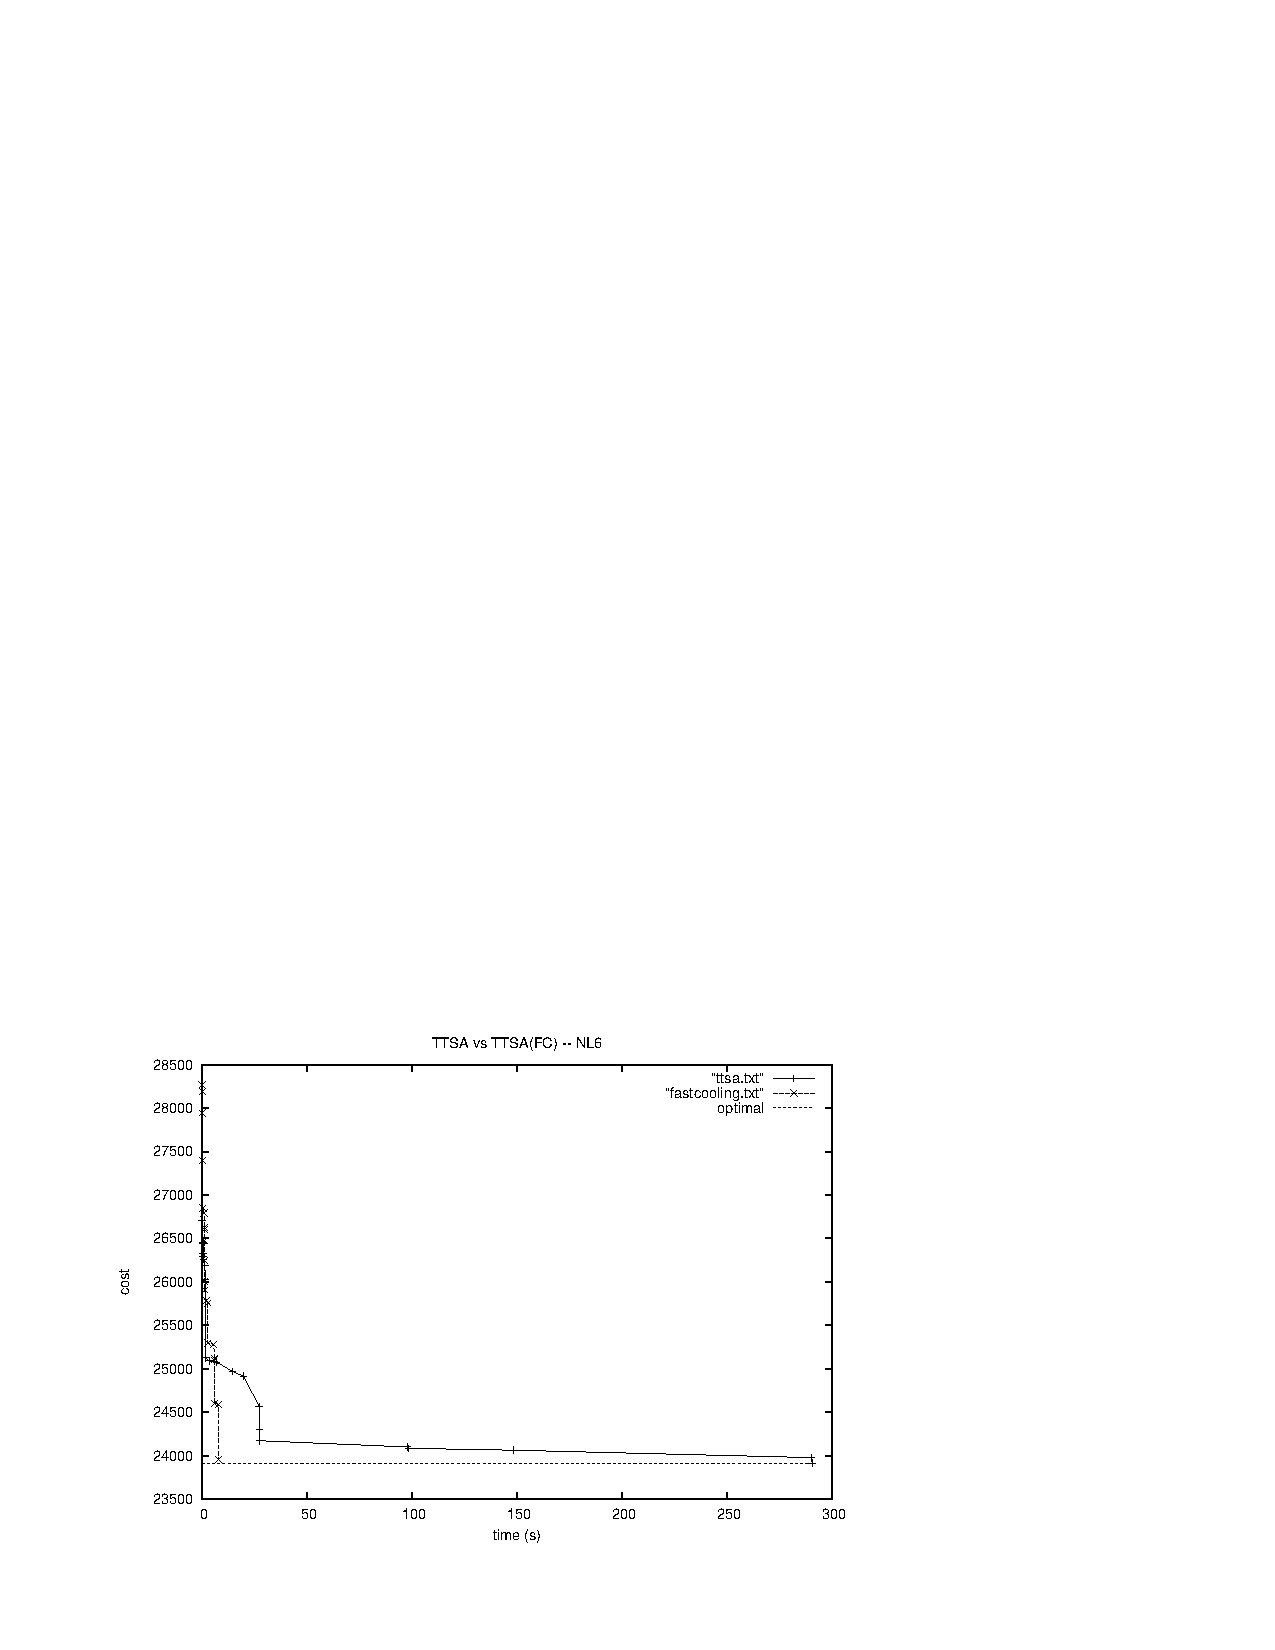
\includegraphics[width=0.75\textwidth,keepaspectratio=true]{nl6_ttsaVSttsaFC}
 \caption{TTSA vs TTSA(FC) NL6.}
 \label{fig:ttsafc6vs}
 \end{figure}

\begin{figure}[hbpt]
\centering
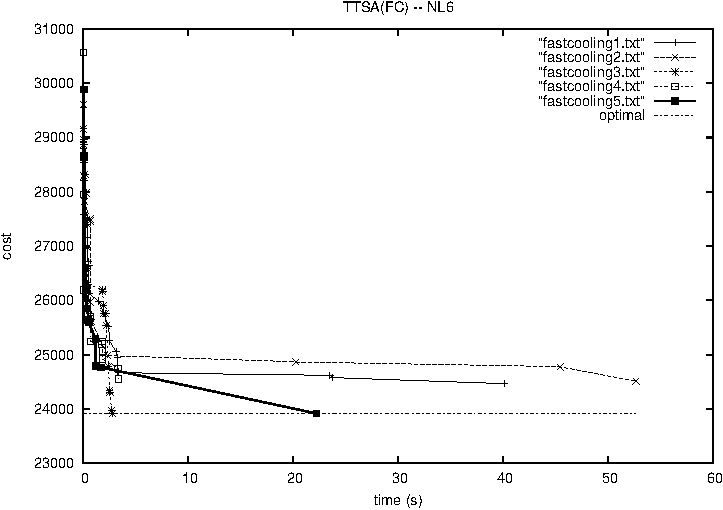
\includegraphics[width=0.75\textwidth,keepaspectratio=true]{fastcoolingNL6}
 \caption{TTSA (FC) NL6.}
 \label{fig:ttsafc6}
 \end{figure}

\begin{figure}[hbpt]
\centering
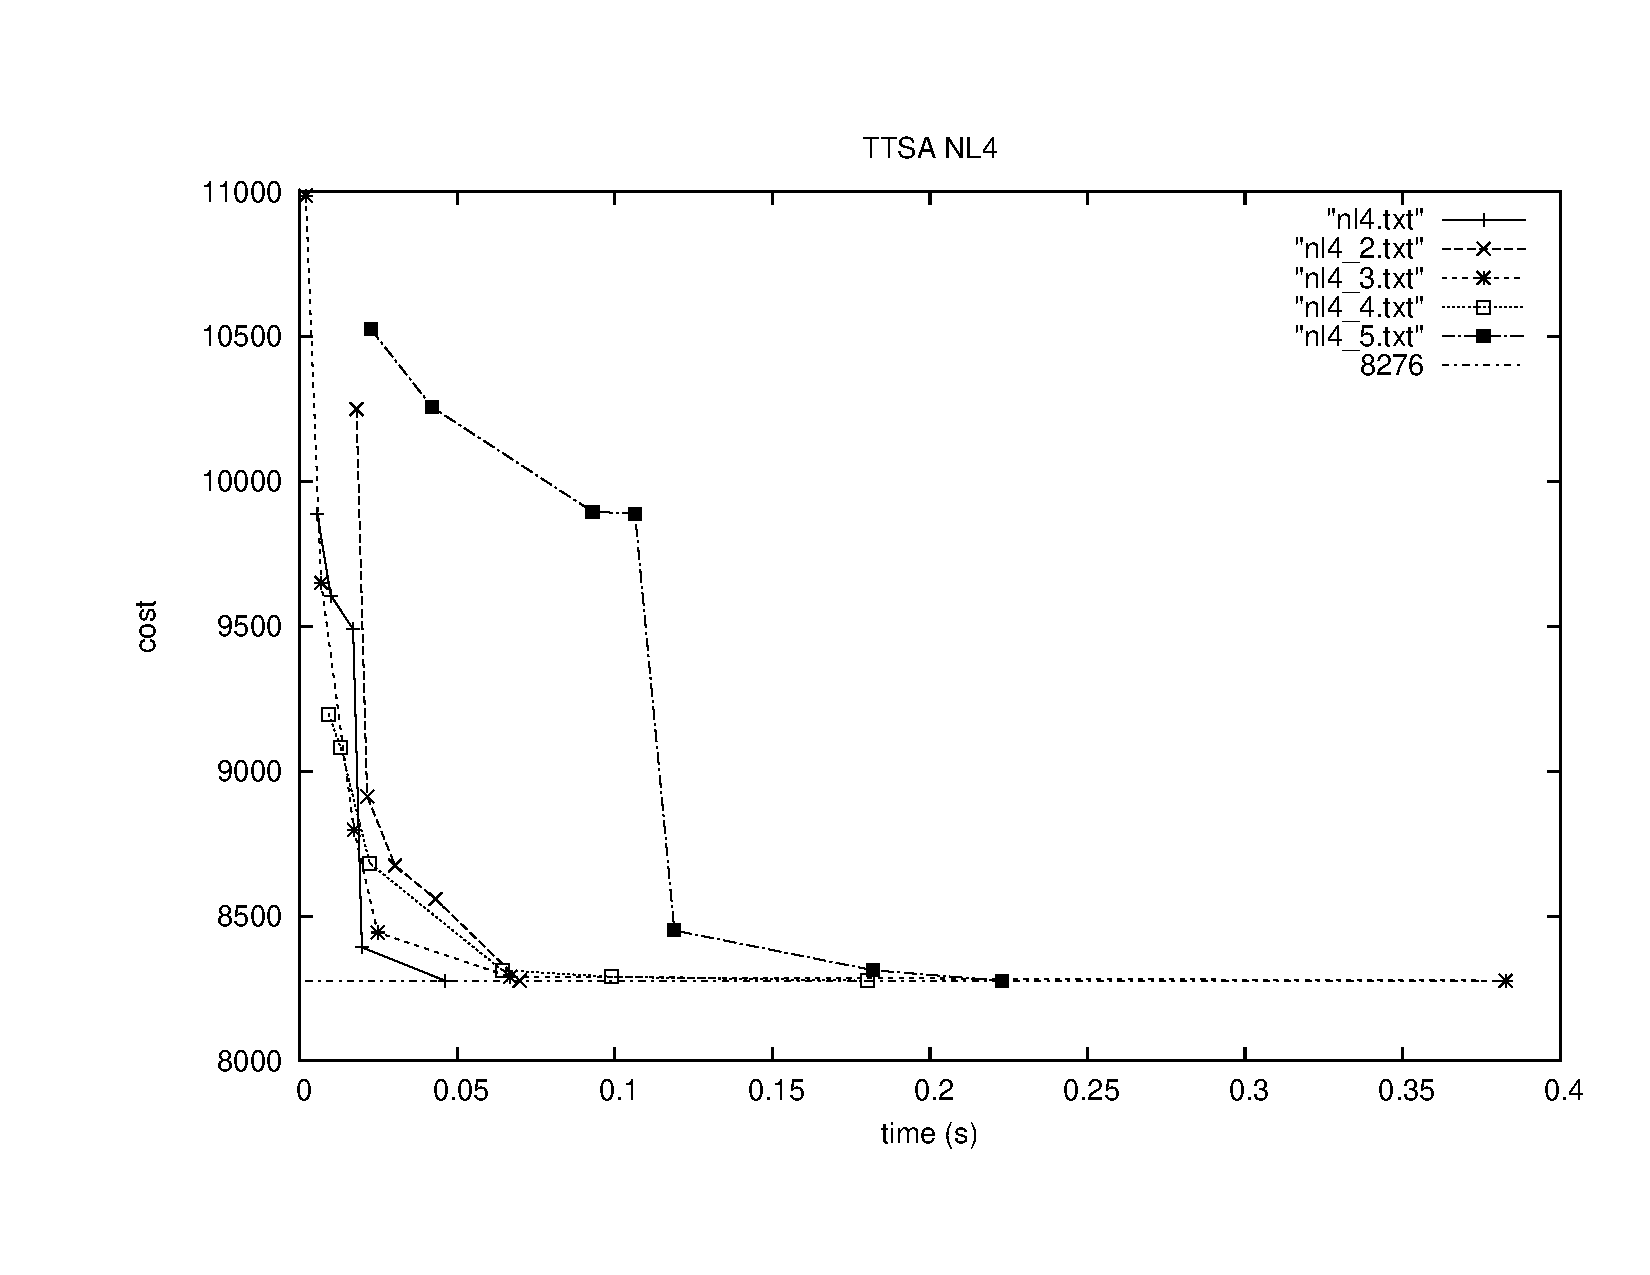
\includegraphics[width=0.75\textwidth,keepaspectratio=true]{ttsaNL4}
 \caption{TTSA NL4.}
 \label{fig:nl4}
 \end{figure}

Het probleem NL4 is triviaal: optimale oplossingen worden in enkele seconden gevonden en de parameters hebben hierbij heel weinig invloed (figuur~\ref{fig:nl4}). Voor NL6 en NL8 werden de optimale oplossingen gevonden; voor NL8 gebeurde dit echter slechts eenmaal en hebben we niet verder geprobeerd wegens tijdsoverwegingen (figuur~\ref{fig:nl8}).

\begin{figure}[hbpt]
\centering
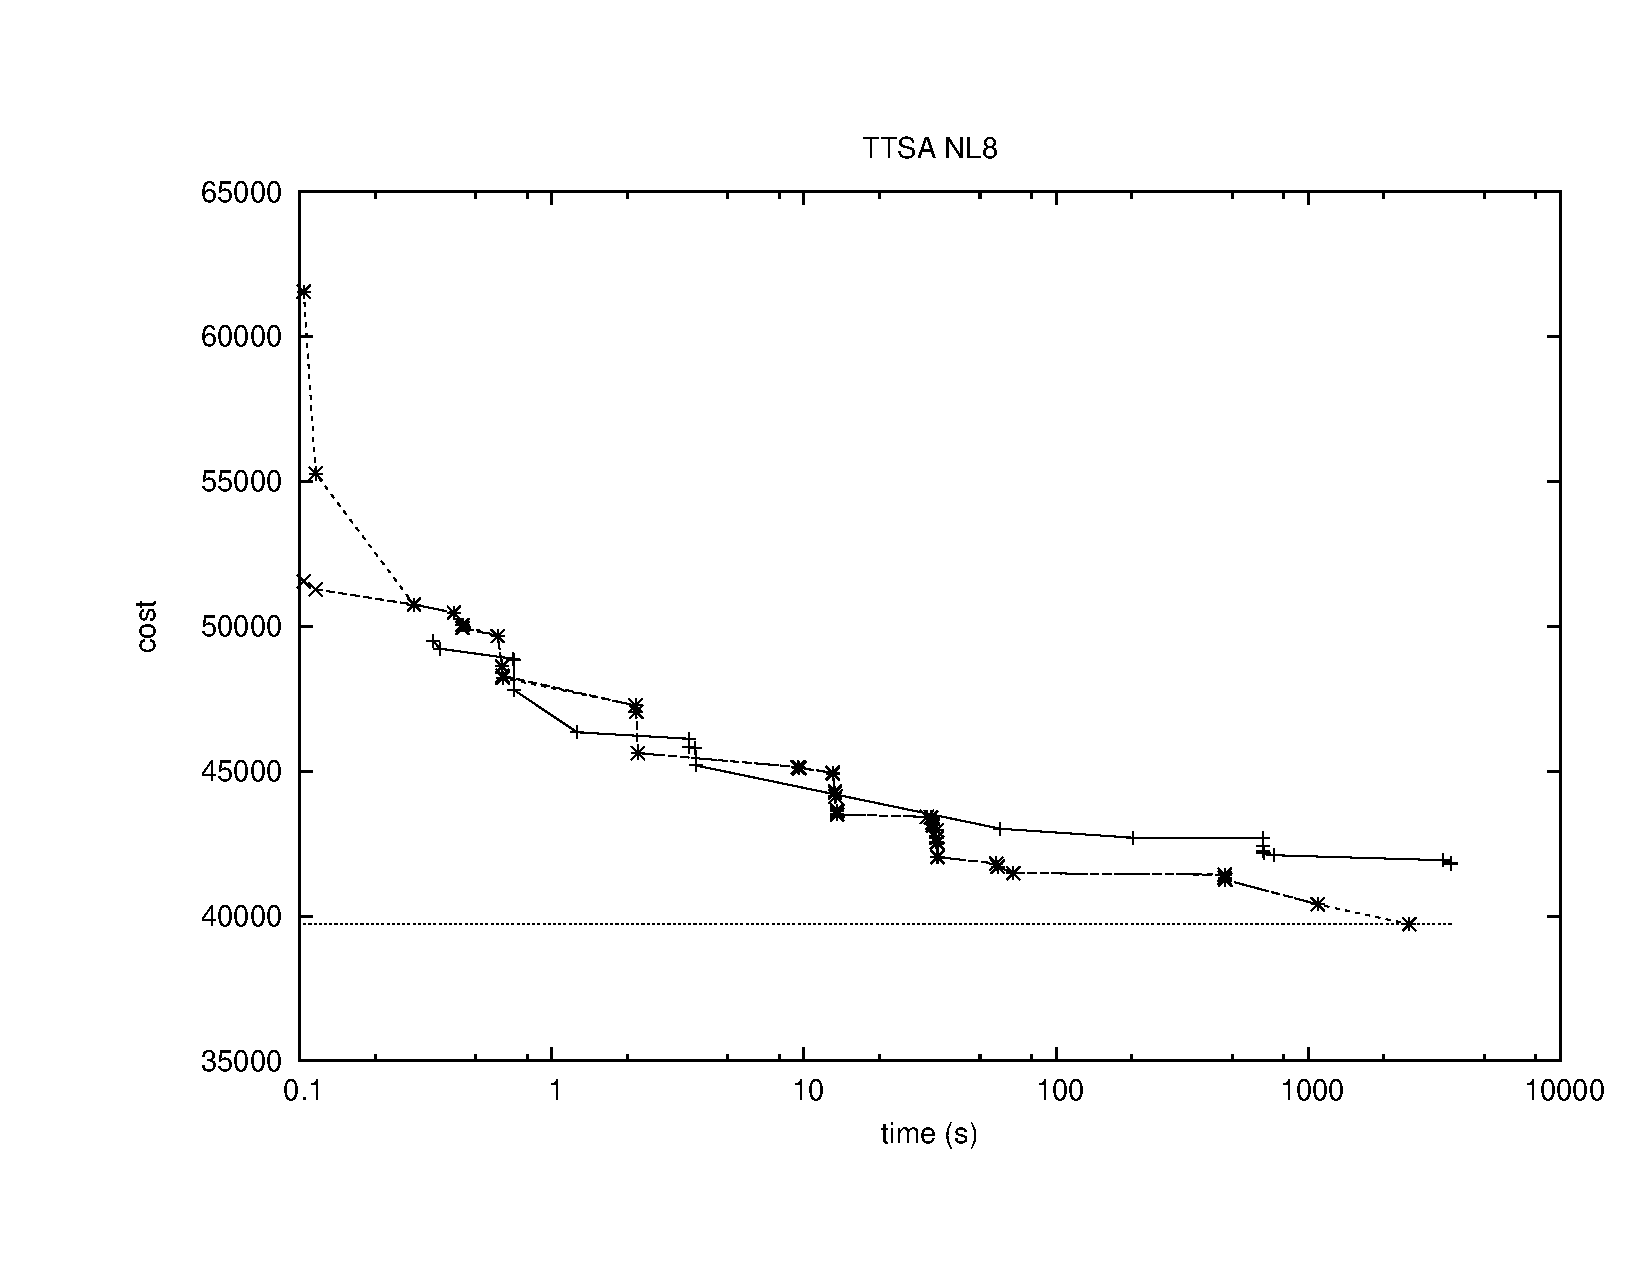
\includegraphics[width=0.8\textwidth,keepaspectratio=true]{ttsaNL8}
 \caption{TTSA NL8.}
 \label{fig:nl8}
 \end{figure}

Figuur~\ref{fig:nl12}, \ref{fig:nl14}, \ref{fig:nl16} toont de resultaten voor respectievelijk NL12, 14 en 16 op een logaritmische tijdsas.

\begin{figure}[hbpt]
\centering
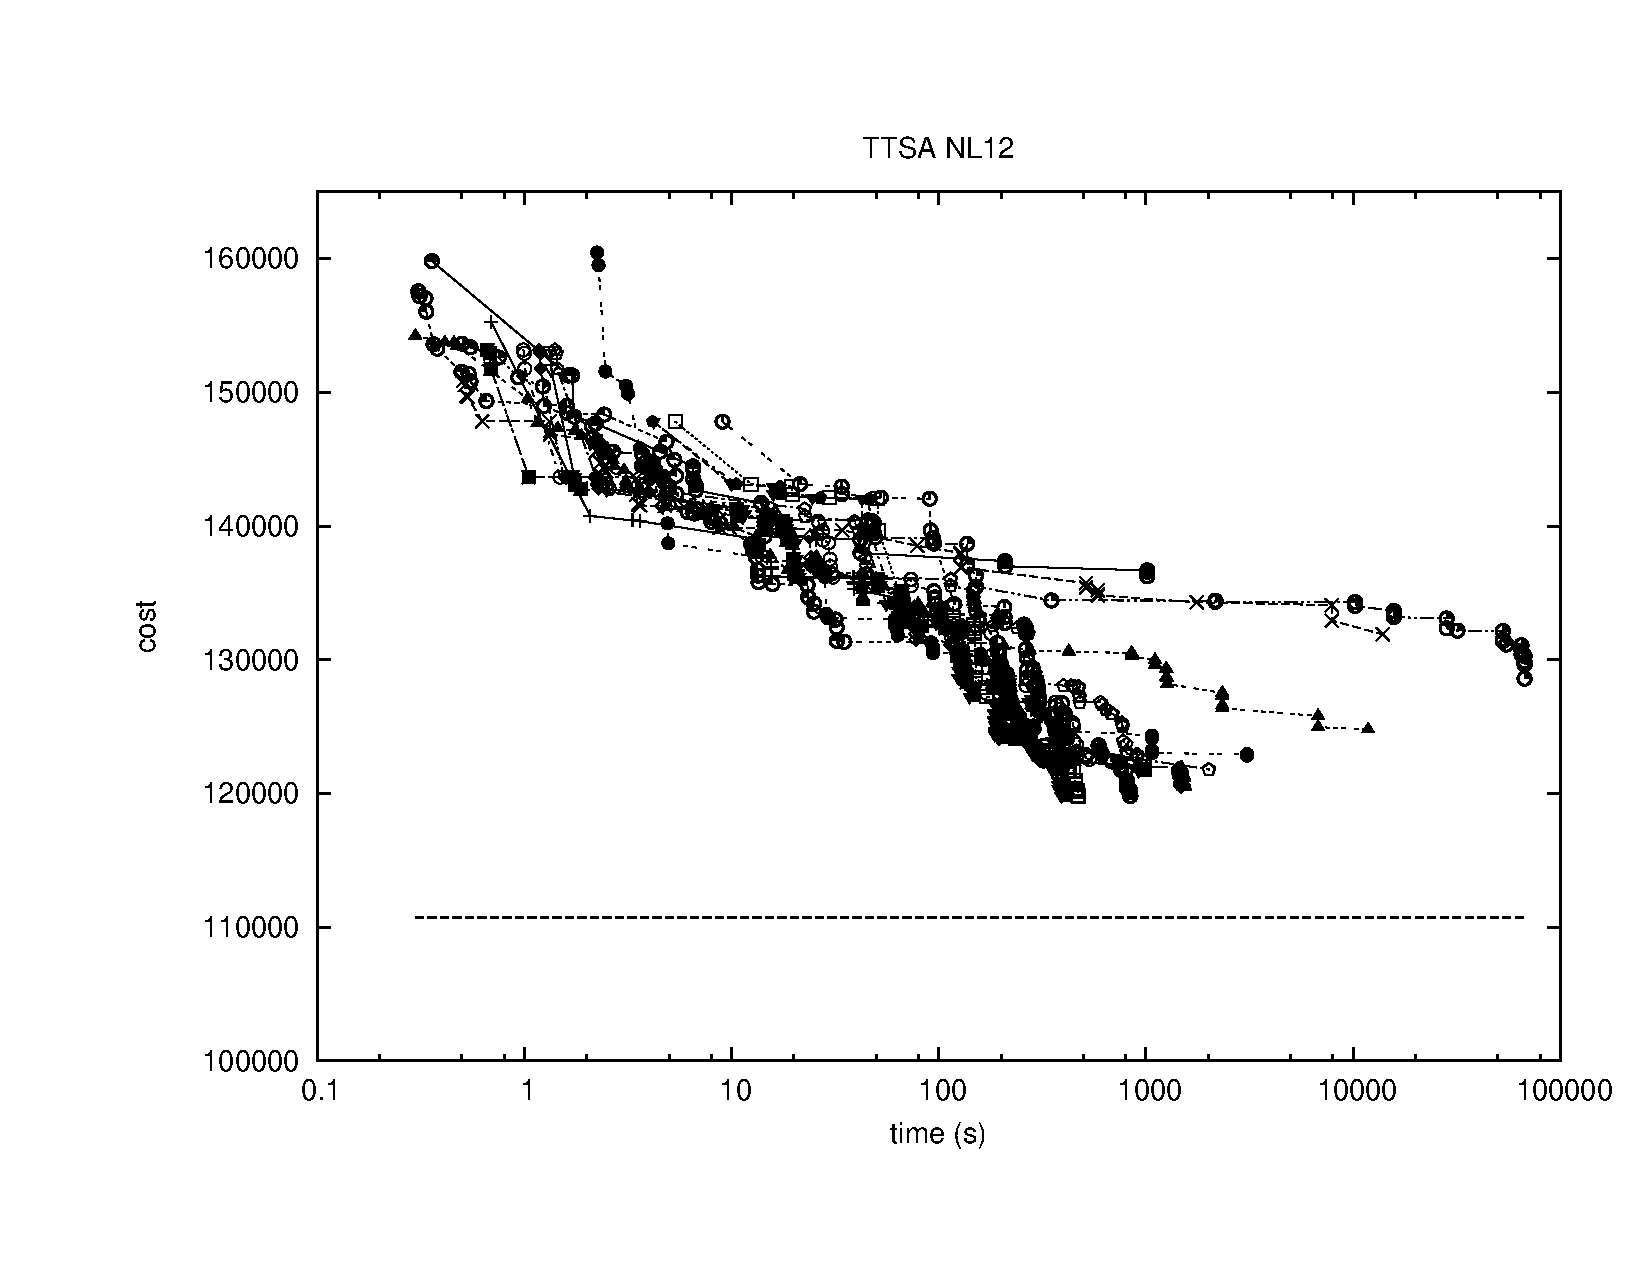
\includegraphics[width=0.8\textwidth,keepaspectratio=true]{ttsaNL12}
 \caption{TTSA NL12 (logaritmische tijdsas).}
 \label{fig:nl12}
 \end{figure}

\begin{figure}[hbpt]
\centering
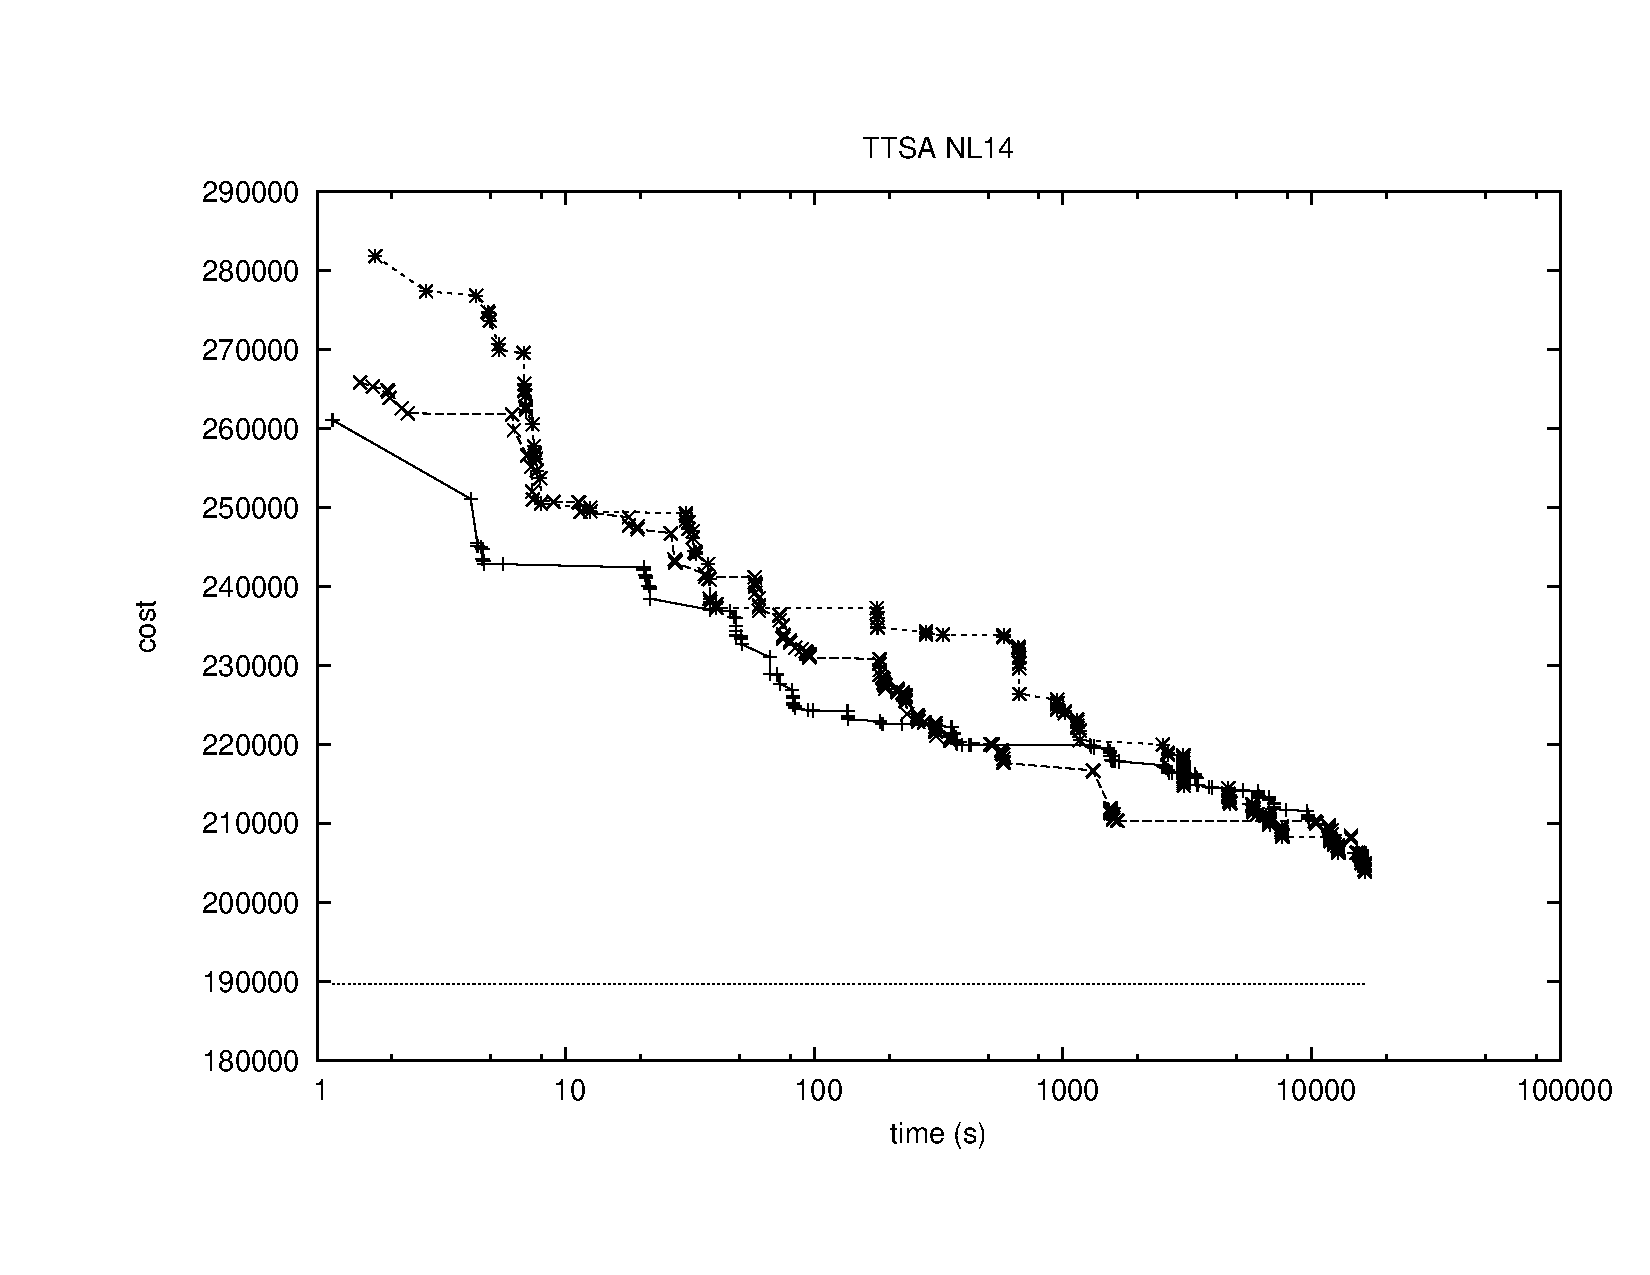
\includegraphics[width=0.8\textwidth,keepaspectratio=true]{ttsaNL14}
 \caption{TTSA NL14 (logaritmische tijdsas).}
 \label{fig:nl14}
 \end{figure}

\begin{figure}[hbpt]
\centering
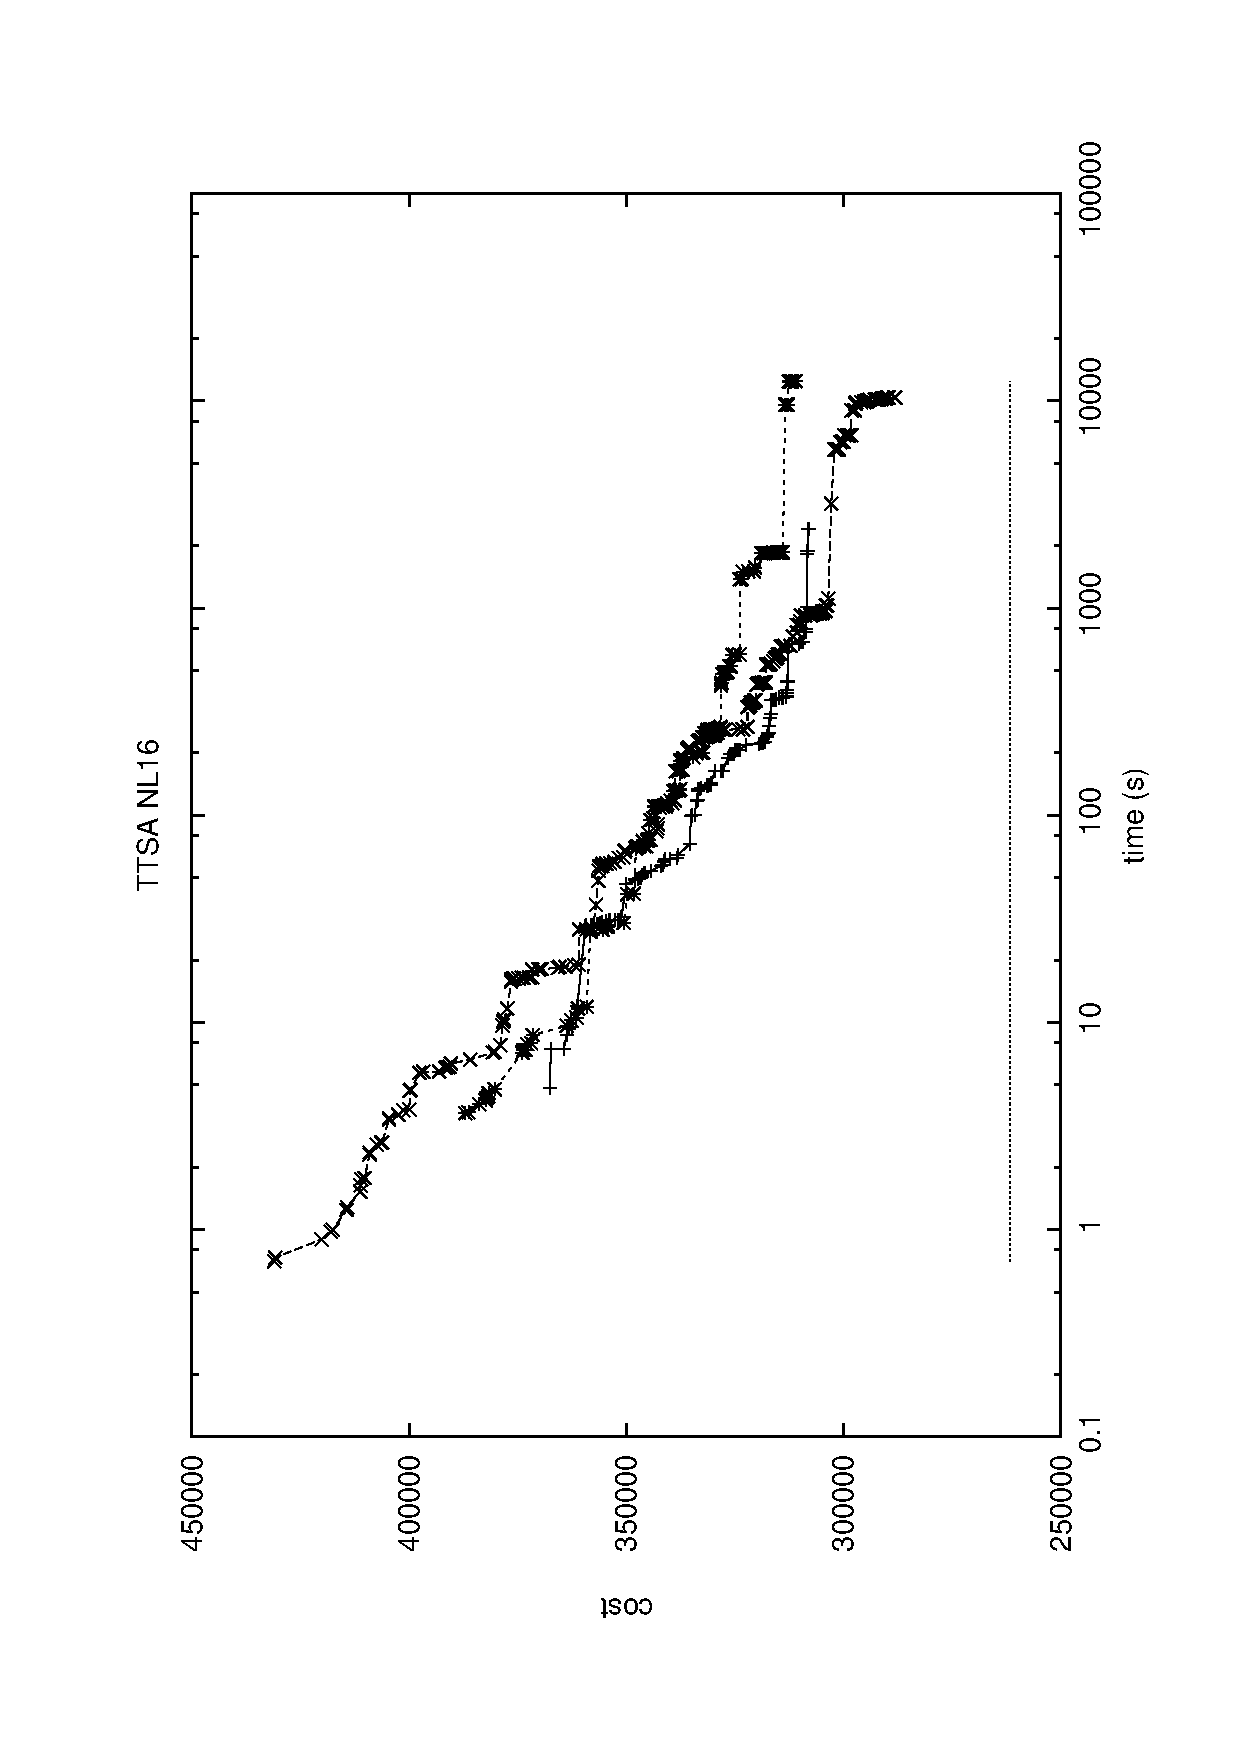
\includegraphics[width=0.8\textwidth,keepaspectratio=true]{ttsaNL16}
 \caption{TTSA NL16 (logaritmische tijdsas).}
 \label{fig:nl16}
 \end{figure}


\begin{table}[hbpt] \centering\footnotesize
\begin{tabular}
{ c   r      S  r    *{3}{S}    r  r          r           r  } \toprule
{$n$} & {cost} & {time (s)} & {$T_0$} & {$\beta$} & {$\delta$} & {$\theta$} & {$maxC$} & {$maxP$} & {$maxR$} & {$w_0$} \\  \midrule

4 & 8276    &	1.2 & 500&	0.99&	1.04&	1.04&	10&	30&	1&	4000 \\
4 & 8276    &	2.2 & 500&	0.99&	1.04&	1.04&	10&	30&	1&	4000\\
4 & 8276     &   0.8 & 500&	0.99&	1.04&	1.04&	10&	30&	1&	4000\\
4 &8276    &	1.2	& 500&	0.99&   1.04&	1.04&	10&	30& 1&	4000\\
4 & 8276    &	1.1	& 500&	0.99&	1.04&	1.04&	10&	30&	1&	4000\\ \addlinespace

6 & 23916 &	225 &	400&	0.99  & 1.04&	1.04&  100 & 100 &	5 &	4000\\
6 & 23916 &	822 &	400&    0.999 &	1.04&	1.04&  5000& 7100&	10&	4000\\
6 & 23916 &	27  &	400&	0.999 &	1.04&	1.04&  100 & 100 &	10&	4000\\
6 & 23916 &	78  &	500&	0.9999&	1.04&   1.04&  50  & 100 &	1 &	4000\\
6 & 24108 & 326 &	500&	0.99  & 1.04&	1.04&  50  & 100 &	1 &	4000     \\
6 & 23916 & 6923&	400&	0.9999& 1.04&	1.04&  5000& 7100&	10&	4000\\
6 & 24070&	371	&400&	0.99&	1.04&	1.04&	100	&100&	3&  4000  \\
6 & 23916&  184	&400&	0.99&	1.04&	1.04&	100 &50 &	2&	4000\\
6 & 24073&	572	&400&	0.99&	1.04&   1.04&	100 &100&	3&	4000\\
6 & 24073&	616	&400&	0.99&	1.04&   1.04&	100	&100&	5&	4000\\
6 & 23916&	225	&400&	0.99&	1.04&   1.04&	100	&100&	5&	4000\\
6 & 23916&	905	&400&	0.99&	1.04&   1.04&	200	&100&	5&	4000\\ \addlinespace

8&40395&	812&	400&	0.99	&1.04	&1.04	&100	&50	&2&	4000\\
8&40340&	1102&	400&	0.99	&1.04	&1.04	&100	&100	&3&	4000\\
8&41126&	301&	400&	0.99	&1.04	&1.04	&100	&100	&1&	4000\\
8&40720&	484&	400&	0.99	&1.04	&1.04	&100	&50	&5&	4000\\
8&41838&	141&	400&	0.99	&1.04	&1.04	&50	&50	&5&	4000\\
8&40228&	270&	400&	0.99	&1.04	&1.04	&50	&100	&3&	4000\\
8&39987&	645&	400&	0.99	&1.04	&1.04	&200	&50	&3&	4000\\
8&40898&	891&	400&	0.99	&1.04	&1.04	&200	&100	&1&	4000\\
8&40018&	213&	400&	0.99	&1.04	&1.04	&100	&50	&3&	4000\\
8&40952&	507&	400&	0.99	&1.04	&1.04	&150	&75	&3&	4000\\
8&39891&	12941&	500&	0.999&	1.04	&1.04	&200	&500	&2&	4000\\
8&39721&	4834&	400&	0.999&	1.04	&1.04	&4000	&7000	&10&	4000\\ \addlinespace

10&66689&	544 &	500&	0.99	&1.04	&1.04	&100	&100	&1	&4000\\
10&66562&	4760&	400&	0.999	&1.04	&1.04	&1000	&100	&7	&4000\\
10&66209&	507	&500&	0.99	&1.04	&1.04	&100	&100	&1	&4000\\
10&65088&	641	&400&	0.99	&1.04	&1.04	&100	&50	&10	&4000\\
10&64379&	414	&400&	0.99	&1.04	&1.04	&100	&50	&7	&4000\\
10&64057&	1903&400&	0.99	&1.04	&1.04	&100	&50	&5	&4000\\ 
10 & 62106 &   417 &  400 & 0.99 & 1.04 & 1.04 & 100 & 50 & 4 & 4000 \\\bottomrule
\end{tabular}
\caption{Experimenten voor NL$n$ instanties\label{tab:experimenten}.}
\end{table}


Tabel~\ref{tab:experimenten} en~\ref{tab:experimenten2} toont alle resultaten en parameters van de uitgevoerde experimenten. Merk op dat de tijd aangeduid de tijd nodig was om de oplossing gegeven in de tabel te zoeken en niet de tijd voor het eindigen van het algoritme.\footnote{Een voorbeeld hiervan is de tijd nodig voor het experiment van NL14 waarbij de oplossing in de tabel na 612\,s werd gevonden; na 6 uur werd geen betere oplossing gevonden en werd het algoritme afgebroken.}

\begin{table}[hbpt] \centering\footnotesize
\begin{tabular}
{ c   r      S  r    *{3}{S}    r  r          r           r  } \toprule
{$n$} & {cost} & {time (s)} & {$T_0$} & {$\beta$} & {$\delta$} & {$\theta$} & {$maxC$} & {$maxP$} & {$maxR$} & {$w_0$} \\  \midrule
12&125684	&15318	&500	&0.99	&1.04	&1.04	&200	&500	&1	&4000\\
12&123701	&4069	&400	&0.99	&1.04	&1.04	&100	&50	&7	&4000\\
12&127697	&1171	&400	&0.99	&1.04	&1.04	&100	&50	&7	&10000\\
12&126360	&3663	&400	&0.9	&1.04	&1.04	&100	&50	&5	&10000\\
12 & 125583    & 65 & 700 & 0.99 & 1.04 & 1.04 & 200 & 100 & 4 & 4000 \\
12 & 121750 & 2606 & 500 & 0.99 & 1.04 & 1.04 & 200 & 100 & 5 & 4000\\
12 & 119807 & 3197 & 500 & 0.99 & 1.04 & 1.04 & 200 & 100 & 5 & 4000\\
12 & 119257 & 4479 & 500 & 0.99 & 1.04 & 1.04 & 200 & 100 & 5 & 4000\\
12 & 118499 & 7450 & 500 & 0.99 & 1.04 & 1.04 & 200 & 100 & 5 & 4000\\
12 & 121750 & 946 & 500 & 0.99 & 1.04 & 1.04 & 200 & 100 & 5 & 4000\\
12 & 121750 & 2618 & 500 & 0.99 & 1.04 & 1.04 & 200 & 100 & 5 & 4000\\
12 & 119807 & 472 & 500 & 0.99 & 1.04 & 1.04 & 200 & 100 & 5 & 4000\\
12 & 120526 & 1524 & 500 & 0.99 & 1.04 & 1.04 & 200 & 100 & 5 & 4000\\
12 & 121750 & 924 & 500 & 0.99 & 1.04 & 1.04 & 200 & 100 & 5 & 4000\\
12 & 119807 & 392 & 500 & 0.99 & 1.04 & 1.04 & 200 & 100 & 5 & 4000\\
12 & 120526 & 1479 & 500 & 0.99 & 1.04 & 1.04 & 200 & 100 & 5 & 4000\\
12 & 121750 & 928 & 500 & 0.99 & 1.04 & 1.04 & 200 & 100 & 5 & 4000\\
12 & 121750 & 2015 & 500 & 0.99 & 1.04 & 1.04 & 200 & 100 & 5 & 4000\\
12 & 119807 & 421 & 500 & 0.99 & 1.04 & 1.04 & 200 & 100 & 5 & 4000\\
12 & 119807 & 844 & 500 & 0.99 & 1.04 & 1.04 & 200 & 100 & 5 & 4000\\
12 & 121750 & 1288 & 500 & 0.99 & 1.04 & 1.04 & 200 & 100 & 5 & 4000\\
12 & 121043 & 1516 & 500 & 0.99 & 1.04 & 1.04 & 200 & 100 & 5 & 4000\\
12 & 120084 & 2850 & 500 & 0.99 & 1.04 & 1.04 & 200 & 100 & 5 & 4000\\ \addlinespace

14 & 217159 &	612 &	500 &	0.999 &	1.04 &	1.04 & 	500 &	100 &	1	& 5000 \\
14 & 210680 &	9727 &	500 &	0.99 &	1.04 &	1.04 & 	200 &	100 &	5	& 4000 \\
14 & 208091 &	14408 &	500 &	0.99 &	1.04 &	1.04 & 	200 &	100 &	5	& 4000 \\
14 & 203979 &	16406 &	600 &	0.99 &	1.03 &	1.03 & 	3000 &	1500 &	10	& 10000 \\ \addlinespace

16& 302671	&5068&	400&	0.99&	1.04&	1.04&	100	&100&	2&	4000\\
16& 288089	&10392	&400&	0.9999&	1.04&	1.04&	10000&	7100&	50&	60000\\\bottomrule
\end{tabular}
\caption{Experimenten voor NL$n$ instanties (\emph{vervolg})\label{tab:experimenten2}.}
\end{table}


 
Tabel~\ref{best} vat de beste gevonden resultaten samen en vergelijkt deze met enerzijds de beste in de paper en anderzijds de beste (gepubliceerde) resultaten op~\cite{website} van 2002 en 2010. Voor de kleinere instanties werden de optimale oplossingen gevonden (die reeds bekend waren). Voor NL12 werd een betere oplossing gevonden dan de best gekende in 2002; onze oplossing is echter nog steeds slechter dan die van de auteurs.



\newpage

\section{Mogelijke verbeteringen}
Enkele mogelijke andere verbeteringen die verder kunnen onderzocht worden, zijn onder andere het gebruik van een andere sublineaire functie, 
een theoretische onderbouwing voor de parameters, de invloed van de random initieel schedules (bv.\ met constraint programming of hill-climbing~\cite{paper2}), betere neighborhoods~\cite{betterneighborhood}, \ldots 

Om de rekentijden te minimaliseren, kunnen parallelle versies van SA onderzocht worden, e.g.~\cite{metaheuristics,parallelSA,parallelSA2}.
Hybride vormen zoals population based SA~\cite{populationSA} en hill-climbing SA~\cite{hybrid} blijken ook beter te werken, maar werden niet onderzocht in dit verslag.


\section{Conclusie}

Met onze implementatie van TTSA hebben we optimale resultaten voor NL4, 6 en 8 kunnen vinden; voor NL10, 12, 14 en 16 enkel suboptimale oplossingen (tabel~\ref{best}). 


 \begin{table}[hbpt]
 \centering 


 \begin{tabular}{c r r r r r r r }\toprule
 $n$ && cost  & && best (2002) &  TTSA (2003) &best (2010)  \\\midrule
 4   && \emph{8276}  & && 8276            &	8276 &8276  \\
 6   && \emph{23916} & && 	23916     &  23916 &23916 \\
 8   && \emph{39721} & &&	  39721   &  39721 &39721  \\
 10  &&  63667     && & 	61608	& 59583 &59436 \\
 12  &&  \emph{118499}     && &	118955	 &112800 &110729 \\
 14  &&   \emph{203979}    && & 205894		&190368 &188728 \\
 16  && 288089   && &       281660          &267194 &261687 \\
 \bottomrule
 
 \end{tabular}


\caption{Beste resultaten gevonden voor NL$n$ instanties met TTSA. 
De voorlaatste kolom geeft de resultaten weer van TTSA (2003)~\cite{paper}; de derde en laatste kolom de beste resultaten zoals op~\cite{website}.\label{best}}
\end{table}

Duidelijke conclusies over de invloed van de parameters hebben we niet kunnen maken: hiervoor zijn te weinig (consistente) experimenten uitgevoerd. De verschillen in de resultaten zijn mogelijk enkel random effecten.

Het is duidelijk dat TTSA oplossingen kan produceren met goede kwaliteit. Nadelen zijn de parameters die enkel empirisch bepaald kunnen worden en de lange rekentijd.
Om de rekentijd te verlagen, blijken fast cooling schedules vrij goed te werken voor redelijk goede oplossingen. 


\clearpage

%% Define a new 'leo' style for the package that will use a smaller font.
\makeatletter
\def\url@leostyle{%
  \@ifundefined{selectfont}{\def\UrlFont{\sf}}{\def\UrlFont{\small\ttfamily}}}
\makeatother
%% Now actually use the newly defined style.
\urlstyle{leo}

\bibliography{biblio}


\end{document}


	

